\documentclass[]{article}
\usepackage{lmodern}
\usepackage{amssymb,amsmath}
\usepackage{ifxetex,ifluatex}
\usepackage{fixltx2e} % provides \textsubscript
\ifnum 0\ifxetex 1\fi\ifluatex 1\fi=0 % if pdftex
  \usepackage[T1]{fontenc}
  \usepackage[utf8]{inputenc}
\else % if luatex or xelatex
  \ifxetex
    \usepackage{mathspec}
  \else
    \usepackage{fontspec}
  \fi
  \defaultfontfeatures{Ligatures=TeX,Scale=MatchLowercase}
\fi
% use upquote if available, for straight quotes in verbatim environments
\IfFileExists{upquote.sty}{\usepackage{upquote}}{}
% use microtype if available
\IfFileExists{microtype.sty}{%
\usepackage{microtype}
\UseMicrotypeSet[protrusion]{basicmath} % disable protrusion for tt fonts
}{}
\usepackage[margin=1in]{geometry}
\usepackage{hyperref}
\hypersetup{unicode=true,
            pdftitle={Pre-reaching infants expect causal agents to reach efficiently},
            pdfauthor={Shari Liu},
            pdfborder={0 0 0},
            breaklinks=true}
\urlstyle{same}  % don't use monospace font for urls
\usepackage{longtable,booktabs}
\usepackage{graphicx,grffile}
\makeatletter
\def\maxwidth{\ifdim\Gin@nat@width>\linewidth\linewidth\else\Gin@nat@width\fi}
\def\maxheight{\ifdim\Gin@nat@height>\textheight\textheight\else\Gin@nat@height\fi}
\makeatother
% Scale images if necessary, so that they will not overflow the page
% margins by default, and it is still possible to overwrite the defaults
% using explicit options in \includegraphics[width, height, ...]{}
\setkeys{Gin}{width=\maxwidth,height=\maxheight,keepaspectratio}
\IfFileExists{parskip.sty}{%
\usepackage{parskip}
}{% else
\setlength{\parindent}{0pt}
\setlength{\parskip}{6pt plus 2pt minus 1pt}
}
\setlength{\emergencystretch}{3em}  % prevent overfull lines
\providecommand{\tightlist}{%
  \setlength{\itemsep}{0pt}\setlength{\parskip}{0pt}}
\setcounter{secnumdepth}{0}
% Redefines (sub)paragraphs to behave more like sections
\ifx\paragraph\undefined\else
\let\oldparagraph\paragraph
\renewcommand{\paragraph}[1]{\oldparagraph{#1}\mbox{}}
\fi
\ifx\subparagraph\undefined\else
\let\oldsubparagraph\subparagraph
\renewcommand{\subparagraph}[1]{\oldsubparagraph{#1}\mbox{}}
\fi

%%% Use protect on footnotes to avoid problems with footnotes in titles
\let\rmarkdownfootnote\footnote%
\def\footnote{\protect\rmarkdownfootnote}

%%% Change title format to be more compact
\usepackage{titling}

% Create subtitle command for use in maketitle
\newcommand{\subtitle}[1]{
  \posttitle{
    \begin{center}\large#1\end{center}
    }
}

\setlength{\droptitle}{-2em}

  \title{Pre-reaching infants expect causal agents to reach efficiently}
    \pretitle{\vspace{\droptitle}\centering\huge}
  \posttitle{\par}
    \author{Shari Liu}
    \preauthor{\centering\large\emph}
  \postauthor{\par}
      \predate{\centering\large\emph}
  \postdate{\par}
    \date{July 31 2018}


\begin{document}
\maketitle

\section{Tables and Figures}\label{tables-and-figures}

\textbf{Table 1.} Summary of conditions, design, and sample sizes of
Experiments 1-5, and SCS Experiments 1-5. Conditions listed under a
single experiment (e.g.~Exp 1 and 3) included random assignment to
condition. For stimuli, see Fig 1. * indicates direct replication.

\begin{longtable}[]{@{}llllllll@{}}
\toprule
Experiment & N & Training & Goal & Habituation & Causal & Mitten &
Stimuli\tabularnewline
\midrule
\endhead
1 & 20 & none & state change & constrained & yes & yes & H1,
T1\tabularnewline
1 & 20 & none & state change & unconstrained & yes & yes & H2,
T1\tabularnewline
2 & 20 & none & state change & constrained & no & yes & H3,
T2\tabularnewline
3* & 26 & none & state change & constrained & yes & yes & H1,
T1\tabularnewline
3* & 26 & none & state change & constrained & no & yes & H3,
T2\tabularnewline
4 & 20 & none & pick up & constrained & yes & yes & H4,
T3\tabularnewline
5 & 20 & none & pick up & constrained & yes & no & H5, T4\tabularnewline
SCS 1 & 20 & effective & pick up & constrained & yes & yes
&\tabularnewline
SCS 2 & 20 & ineffective & pick up & constrained & yes & yes
&\tabularnewline
SCS 3 & 20 & none & pick up & constrained & yes & yes &\tabularnewline
SCS 4* & 26 & effective & pick up & constrained & yes & yes
&\tabularnewline
SCS 5 & 26 & effective & pick up & unconstrained & yes & yes
&\tabularnewline
\bottomrule
\end{longtable}

\begin{center}\rule{0.5\linewidth}{\linethickness}\end{center}

\begin{figure}[htbp]
\centering
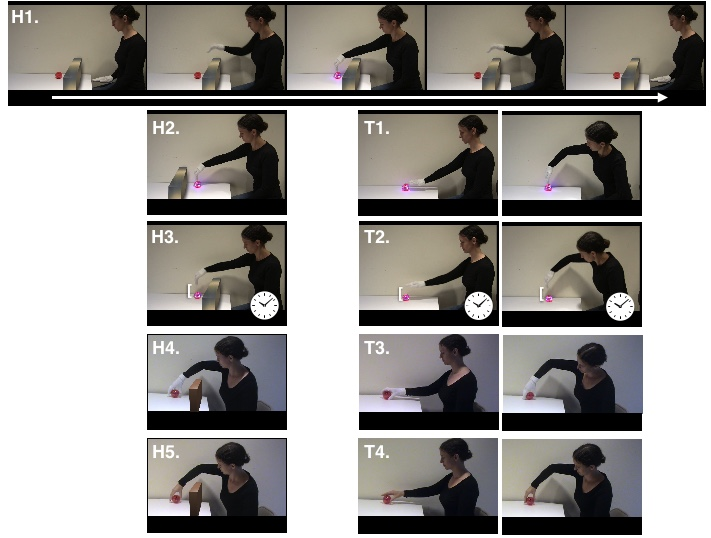
\includegraphics{/Users/shariliu/Documents/HarvardLDS/Studies/LUMI/github/analyses/fig1.jpeg}
\caption{\textbf{Figure 1.} Still frames from videos shown to
participants in Experiments 1-5, including stimuli from habituation
(H1-H5) and test (T1-T4). In each video, a person reached for and caused
a change in an object (H1-H3, T1-T2), or picked up the object (H4-H5,
T3-T4), over a barrier (H1- H2, H4-H5) or over empty space (H2, T1-T4),
and either acted on the object by contacting it (H1-H2, H4-H5, T1,
T3-T4) or produced the same effect from a distance of 50 pixels, after a
0.5s delay (H3, T2). During test (T1-T4), the person either reached
directly for the object (T1-T4, left panel), or in a curvilinear fashion
(T1-T4, right panel).}
\end{figure}

\begin{center}\rule{0.5\linewidth}{\linethickness}\end{center}

A. 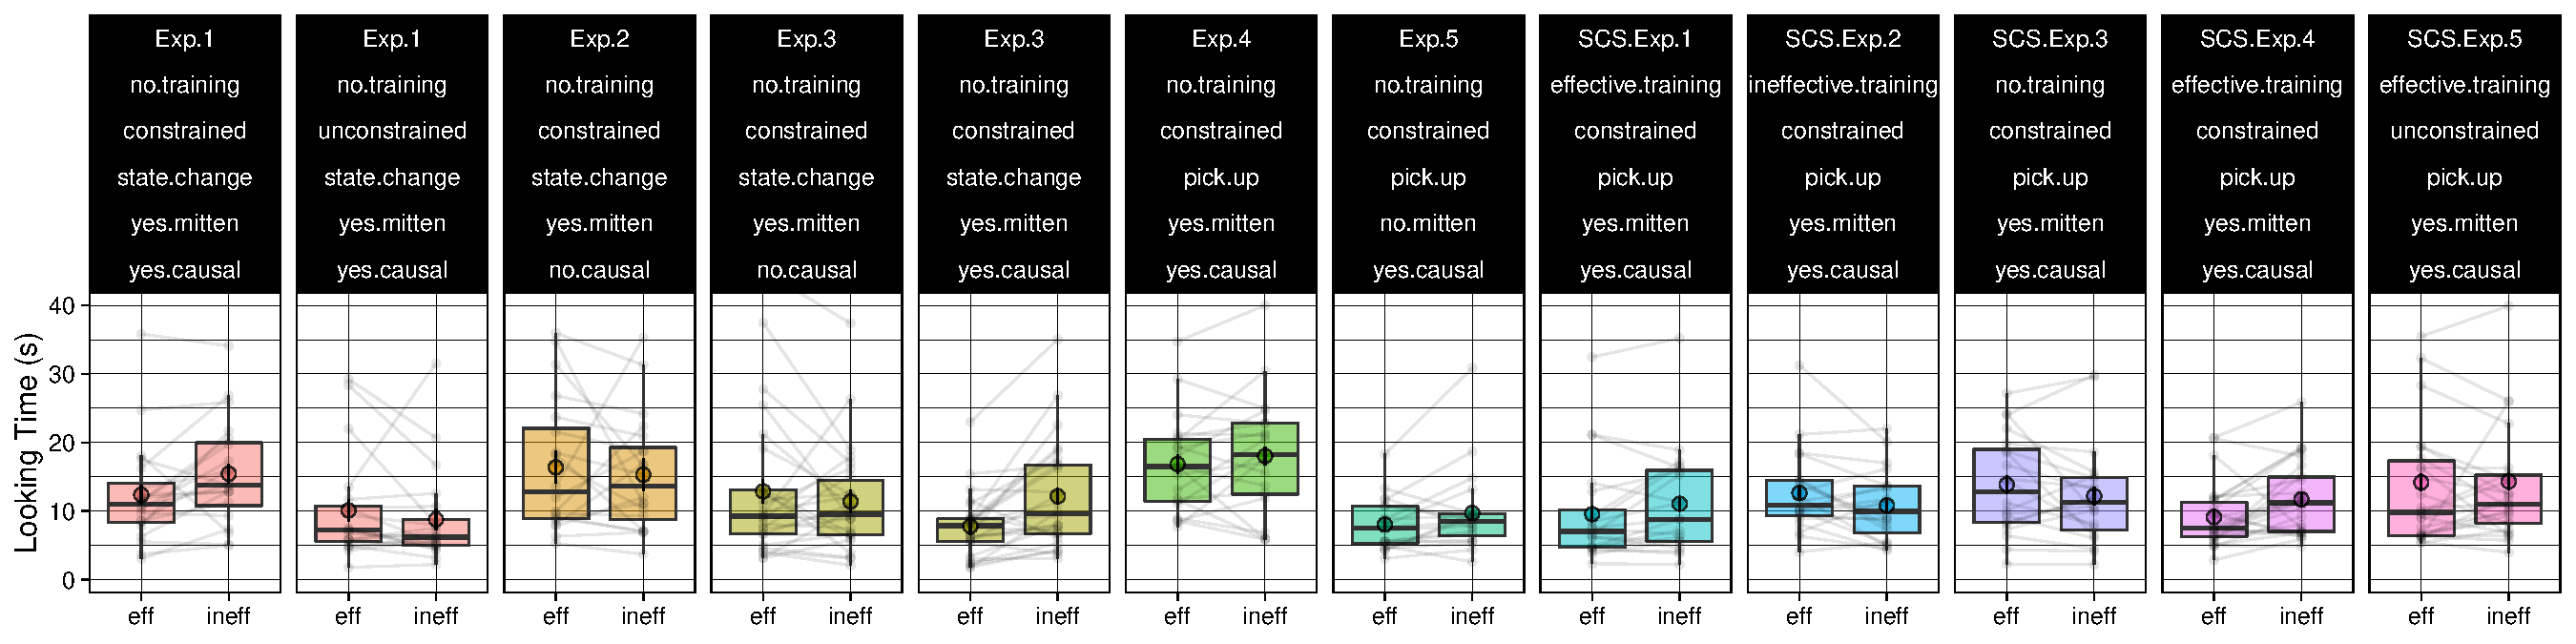
\includegraphics{lumi_analysis_files/figure-latex/fig2a-1.pdf} B.
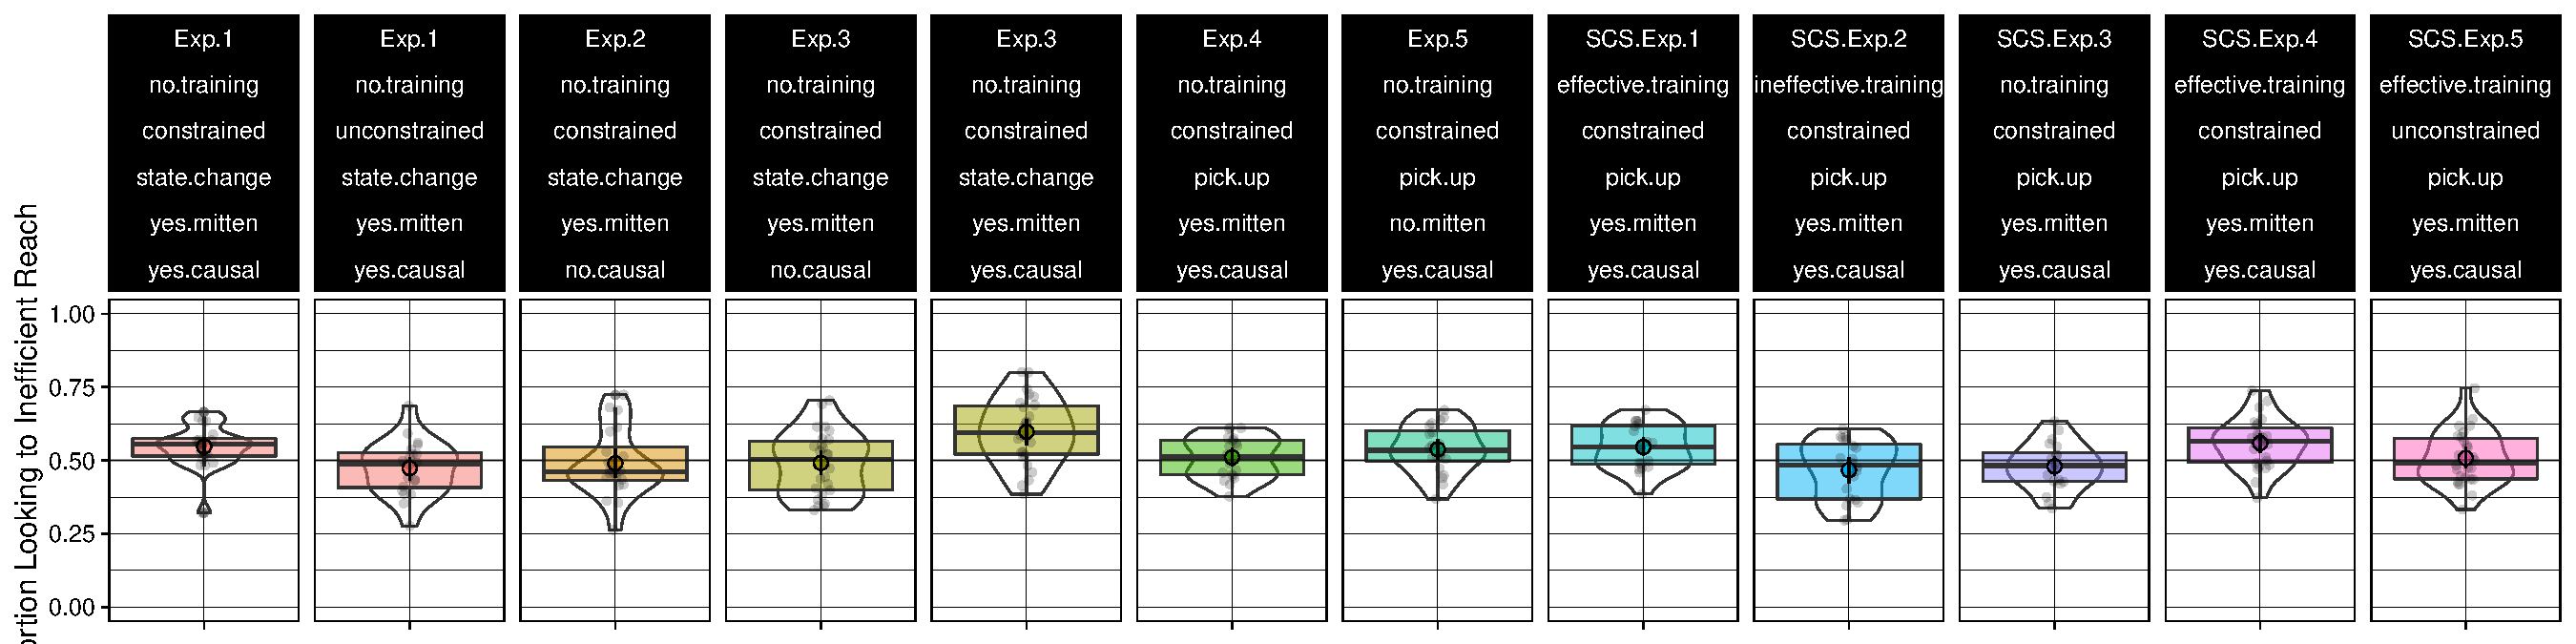
\includegraphics{lumi_analysis_files/figure-latex/fig2b-1.pdf}

\textbf{Figure 2.} Looking time in (A) seconds towards the efficient
versus inefficient reach, and (B) proportion looking towards the
inefficient reach at test across Experiments 1-5 (\emph{n}=152) and
across Experiments 1-5 in Skerry et al. (2013) (\emph{n}=112). Labels
above each panel list the experiment name (Exp. 1-5, SCS Exp. 1-5), type
of motor training (none, sticky, or not.sticky mittens), type of
habituation (constrained or unconstrained), goal (state.change or
pick.up), whether her actions appeared to be causal (yes.causal or
no.causal), and whether the actress wore a mitten (yes.mitten or
no.mitten). Error bars around means indicate within-subjects 95\%
confidence intervals (A) and bootstrapped 95\% confidence intervals (B).
Individual points (B) or pairs of points (A) indicate data from a single
participant. Horizontal bars within boxes indicate medians, and boxes
indicate the middle 2 quartiles of data. Violin plots in (B) indicate
distribution of data, area scaled proportionally to the number of
observations.

\begin{center}\rule{0.5\linewidth}{\linethickness}\end{center}

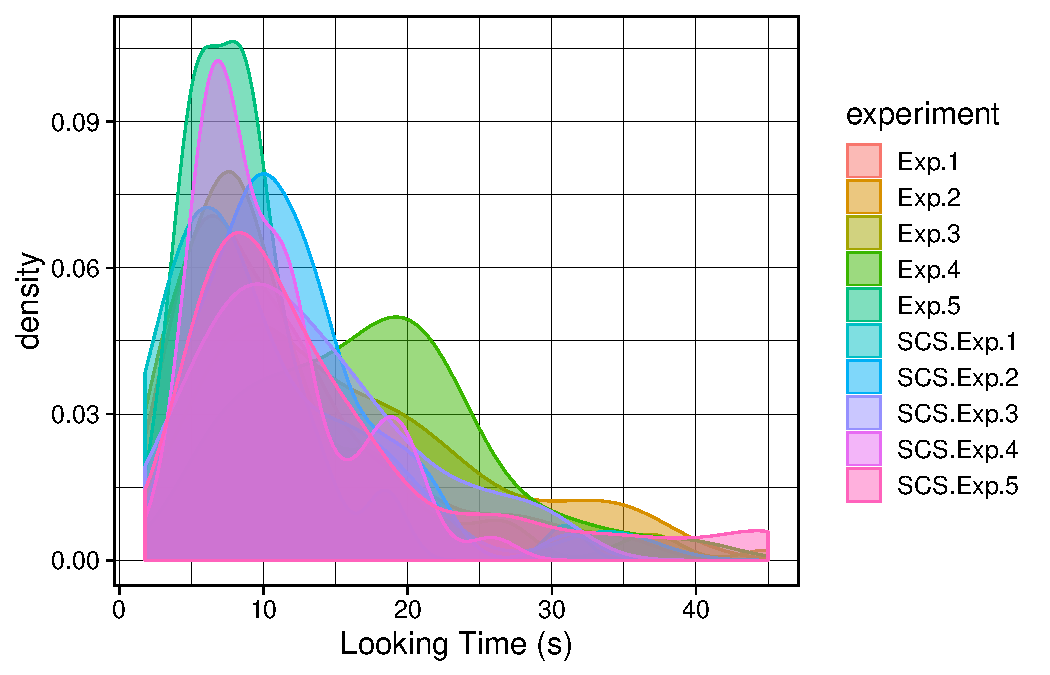
\includegraphics{lumi_analysis_files/figure-latex/figS1-1.pdf}

\textbf{Figure S1.} Density plot of looking times during test across
Experiments 1-5, and Experiments 1-5 from Skerry et al. (2013) (N=264).
Maximum-likelihood fitting revealed that the lognormal distribution (log
likelihood=-1720.509) provides a better fit to these data than the
normal distribution (log likelihood=-1842.196).

\begin{center}\rule{0.5\linewidth}{\linethickness}\end{center}

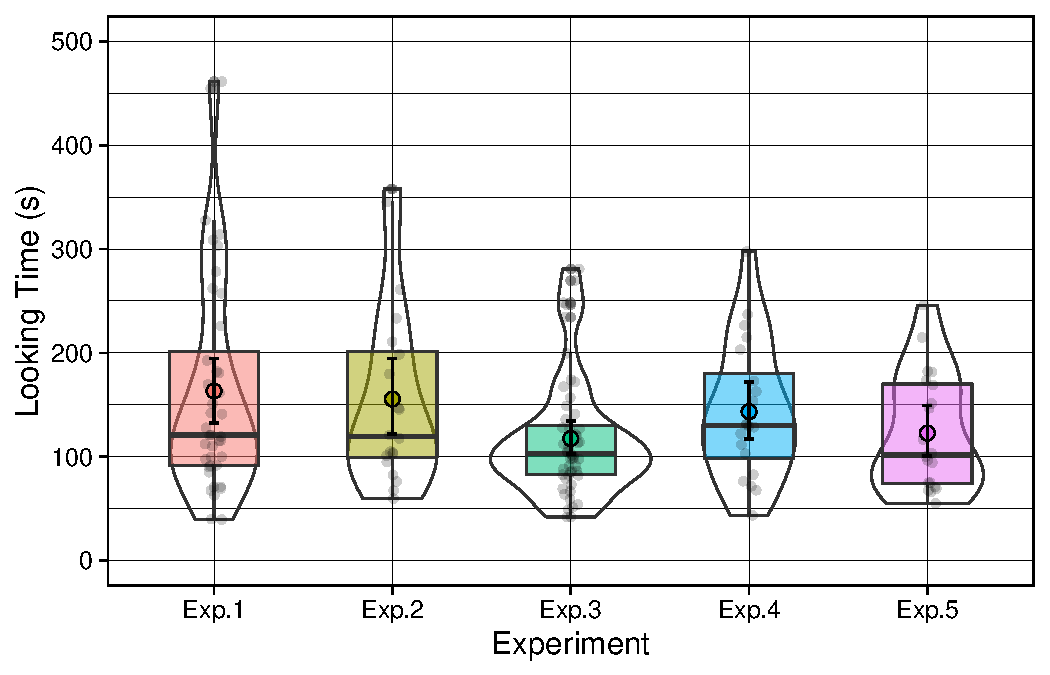
\includegraphics{lumi_analysis_files/figure-latex/figS2-1.pdf}

\textbf{Figure S2.} Total looking time in seconds during habituation
across Experiment 1-5. Error bars around means indicate bootstrapped
95\% confidence intervals. Individual points indicate data from a single
participant. Horizontal bars within boxes indicate medians, and boxes
indicate the middle 2 quartiles of data. Violin plots in indicate
distribution of data, area scaled proportionally to the number of
observations.

\begin{center}\rule{0.5\linewidth}{\linethickness}\end{center}

\section{Results}\label{results}

\subsection{Reliability}\label{reliability}

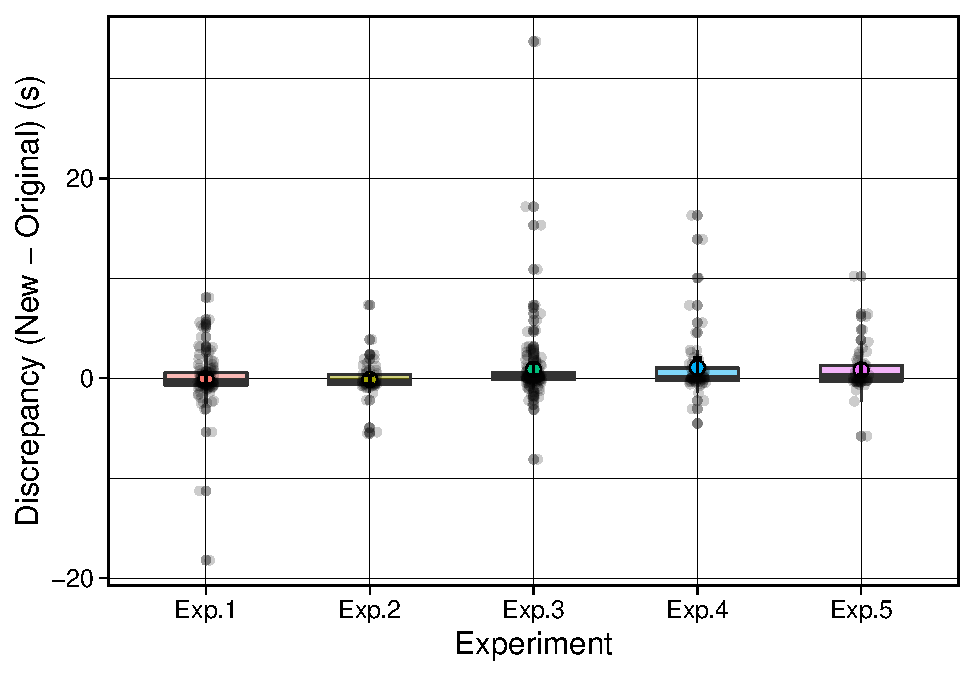
\includegraphics{lumi_analysis_files/figure-latex/rel_plot-1.pdf}

\textbf{Figure S3.} Discrepancy between original and new coding of
looking times during test trials in seconds.

\begin{center}\rule{0.5\linewidth}{\linethickness}\end{center}

To assess reliability, 50\% of test trials from participants across
Experiments 1-5 (132 participants, 456 trials) were randomly selected
and coded by additional researchers who were unaware of experimental
condition, and test trial order. The intraclass correlation coefficient
(ICC) between the original data, and this newly coded data, was 0.968
{[}0.955, 0.978{]}, 0.963 {[}0.938, 0.977{]}, 0.936 {[}0.911, 0.954{]},
0.969 {[}0.946, 0.982{]}, 0.969 {[}0.943, 0.982{]}, for Experiments 1
through 5, respectively.

\subsection{Exclusion info}\label{exclusion-info}

\begin{longtable}[]{@{}lllllll@{}}
\toprule
\begin{minipage}[b]{0.08\columnwidth}\raggedright\strut
Experiment\strut
\end{minipage} & \begin{minipage}[b]{0.07\columnwidth}\raggedright\strut
Fussiness\strut
\end{minipage} & \begin{minipage}[b]{0.12\columnwidth}\raggedright\strut
Inattentiveness\strut
\end{minipage} & \begin{minipage}[b]{0.17\columnwidth}\raggedright\strut
Caregiver Interference\strut
\end{minipage} & \begin{minipage}[b]{0.19\columnwidth}\raggedright\strut
Experimenter/Coding Error\strut
\end{minipage} & \begin{minipage}[b]{0.13\columnwidth}\raggedright\strut
Technical Failure\strut
\end{minipage} & \begin{minipage}[b]{0.04\columnwidth}\raggedright\strut
Total\strut
\end{minipage}\tabularnewline
\midrule
\endhead
\begin{minipage}[t]{0.08\columnwidth}\raggedright\strut
Exp.1\strut
\end{minipage} & \begin{minipage}[t]{0.07\columnwidth}\raggedright\strut
9\strut
\end{minipage} & \begin{minipage}[t]{0.12\columnwidth}\raggedright\strut
5\strut
\end{minipage} & \begin{minipage}[t]{0.17\columnwidth}\raggedright\strut
1\strut
\end{minipage} & \begin{minipage}[t]{0.19\columnwidth}\raggedright\strut
6\strut
\end{minipage} & \begin{minipage}[t]{0.13\columnwidth}\raggedright\strut
3\strut
\end{minipage} & \begin{minipage}[t]{0.04\columnwidth}\raggedright\strut
24\strut
\end{minipage}\tabularnewline
\begin{minipage}[t]{0.08\columnwidth}\raggedright\strut
Exp.2\strut
\end{minipage} & \begin{minipage}[t]{0.07\columnwidth}\raggedright\strut
0\strut
\end{minipage} & \begin{minipage}[t]{0.12\columnwidth}\raggedright\strut
0\strut
\end{minipage} & \begin{minipage}[t]{0.17\columnwidth}\raggedright\strut
0\strut
\end{minipage} & \begin{minipage}[t]{0.19\columnwidth}\raggedright\strut
2\strut
\end{minipage} & \begin{minipage}[t]{0.13\columnwidth}\raggedright\strut
0\strut
\end{minipage} & \begin{minipage}[t]{0.04\columnwidth}\raggedright\strut
2\strut
\end{minipage}\tabularnewline
\begin{minipage}[t]{0.08\columnwidth}\raggedright\strut
Exp.3\strut
\end{minipage} & \begin{minipage}[t]{0.07\columnwidth}\raggedright\strut
6\strut
\end{minipage} & \begin{minipage}[t]{0.12\columnwidth}\raggedright\strut
0\strut
\end{minipage} & \begin{minipage}[t]{0.17\columnwidth}\raggedright\strut
0\strut
\end{minipage} & \begin{minipage}[t]{0.19\columnwidth}\raggedright\strut
2\strut
\end{minipage} & \begin{minipage}[t]{0.13\columnwidth}\raggedright\strut
0\strut
\end{minipage} & \begin{minipage}[t]{0.04\columnwidth}\raggedright\strut
8\strut
\end{minipage}\tabularnewline
\begin{minipage}[t]{0.08\columnwidth}\raggedright\strut
Exp.4\strut
\end{minipage} & \begin{minipage}[t]{0.07\columnwidth}\raggedright\strut
7\strut
\end{minipage} & \begin{minipage}[t]{0.12\columnwidth}\raggedright\strut
0\strut
\end{minipage} & \begin{minipage}[t]{0.17\columnwidth}\raggedright\strut
0\strut
\end{minipage} & \begin{minipage}[t]{0.19\columnwidth}\raggedright\strut
2\strut
\end{minipage} & \begin{minipage}[t]{0.13\columnwidth}\raggedright\strut
0\strut
\end{minipage} & \begin{minipage}[t]{0.04\columnwidth}\raggedright\strut
7\strut
\end{minipage}\tabularnewline
\begin{minipage}[t]{0.08\columnwidth}\raggedright\strut
Exp.5\strut
\end{minipage} & \begin{minipage}[t]{0.07\columnwidth}\raggedright\strut
6\strut
\end{minipage} & \begin{minipage}[t]{0.12\columnwidth}\raggedright\strut
0\strut
\end{minipage} & \begin{minipage}[t]{0.17\columnwidth}\raggedright\strut
0\strut
\end{minipage} & \begin{minipage}[t]{0.19\columnwidth}\raggedright\strut
1\strut
\end{minipage} & \begin{minipage}[t]{0.13\columnwidth}\raggedright\strut
2\strut
\end{minipage} & \begin{minipage}[t]{0.04\columnwidth}\raggedright\strut
9\strut
\end{minipage}\tabularnewline
\bottomrule
\end{longtable}

\begin{center}\rule{0.5\linewidth}{\linethickness}\end{center}

\subsection{Experiment 1}\label{experiment-1}

In Experiment 1 (N=40; 20 per condition), we asked whether 3-month-old
infants expect a person to reach out and cause an object to change state
efficiently. Half of infants were randomly assigned to habituate to a
person who reached over a barrier (H1) and appeared to cause an object
to light up by touching it, and then tested on efficient and inefficient
reaches without the barrier (T1). The other half of infants habituated
to the same reaches except that the barrier was located beyond the goal
object, out of the person's way (H2), and viewed the same test events
Infants responded differently to the test events across these two
habituation conditions, {[}-0.657, -0.115{]}, B=-0.386, ß=0.156, 0.398,
-0.412, -0.596, p=0.007, mixed effects model with fixed interaction
between habituation and test event and random intercept for
participants. We found that infants looked longer at the inefficient
action (M=15.448s, SD=2.942) than the efficient action (M=12.368s,
SD=2.942), {[}-0.451, -0.065{]}, B=-0.258, ß=-0.398, p=0.01. And
critically, this looking preference cannot be attributed to low-level
preferences for the curvilinear reach, because infants who were randomly
assigned to habituate to identical videos without the barrier in the way
(H2) looked equally to the inefficient (M=8.788s, SD=3.301) and
efficient (M=10.104s, SD=3.301) actions, {[}-0.065, 0.321{]}, B=0.128,
ß=0.198, p=0.186.

\subsection{Experiment 2}\label{experiment-2}

In Experiment 2 (N=20), we asked whether infants' sensitivity to the
efficiency of this action depends their construal of the person as a
causal agent (an agent contacting an object, thereby changing its state)
or on lower-level scene features (an agent reaching towards a toy that
lights up), by manipulating the spatiotemporal contingency of this
action. In Experiment 2, pre-registered at \url{https://osf.io/a5byn/},
infants were habituated to videos identical to H1, except that the
person's hand stopped 50 pixels away from the object, and the object
changed state after a 0.5 delay (H3). At test, the person reached
efficiently or inefficiently in the absence of the barrier with the same
spatiotemporal gap (T2). This manipulation was inspired by past studies
of causal perception (cite, cite), and asks whether infants' analysis of
the causal structure of an action is critical to their understanding of
this action as intentional. We found that infants looked equally between
the efficient (M=16.38s, SD=5.024) and inefficient (M=15.306s, SD=5.024)
reach (T2), B=-0.055, p=0.649, mixed effects model with trial type as
fixed effect and participants as a random intercept, a result that
differed from infants' responses to causally contingent videos, B=0.313,
p=0.049, mixed effects model with fixed interaction between causality
and trial type.

\subsection{Experiment 3}\label{experiment-3}

Experiment 3 (N=52; 26 per condition) attempts to replicates the
findings from Experiments 1 and 2 by asking whether infants only expect
causally effective reaches to be efficient, relative to the same actions
that are not spatiotemporally contingent. In this experiment,
pre-registered at \url{https://osf.io/f2hvd/}, we randomly assigned
infants to H1 and T1, or H2 and T2, which enables us to stringently
compare infants' responses to the test displays as a function of causal
information. Infants again looked to the events differently depending on
whether the events were causal, B=0.5, p=0.003, mixed effects model with
fixed interaction of causality and test event. Like in Experiment 1,
infants looked longer at the inefficient reach (M=12.166s, SD=2.996)
versus the efficient reach (M=7.791s, SD=2.996) when the person's
actions were causally effective, B=-0.436, p=3\times 10\^{}\{-4\}, and
as in Experiment 3, infants looked equally to the inefficient
(M=11.395s, SD=4.17) and efficient (M=12.888s, SD=4.17) reach when her
actions were causally non-contingent, B=0.064, p=0.567. Together,
Experiments 1-3 show that pre-reaching infants apply the principle of
efficiency (Gergely \& Csibra, 2003) to reaching actions that they
themselves have never experienced, and that they only apply this
principle to actions that appear to cause changes in the world.

\subsection{Experiments 4 and 5}\label{experiments-4-and-5}

Why do infants succeed here without motor training, and fail in Skerry
et al. (2013)? One possibility is that pre-reaching infants struggle to
understand the causal structure of reaching for and retrieving an object
without the relevant motor experience. Another possibility is that
pre-reaching infants do not interpret the reach of a mittened hand, one
that looks different from most hands they see, as intentional without
the relevant experience of observing and experiencing their own mittened
hands act causally during training (cite Woodward glove?). To test for
this second possibility, we ran two additional experiments. In
Experiment 4 (N=20), infants were habituated and tested on events very
similar to those from Skerry (H4, T3), where a person reaches for and
picks up an object while wearing a white mitten. In Experiment 5 (N=20),
infants saw almost identical videos to those from Experiment 4 except
that the person reached with a bare hand (H5, T4). \footnote{Experiments
  4 and 5 were run before Exp 2 and 3, and before our lab began to
  pre-register experiments. As in Experiments 2 and 3, sample sizes,
  analyses, and exclusionary criteria for these 2 experiments were set
  prior to data collection.}

We found that infants looked marginally longer at the inefficient
(M=9.715, SD=2.118) than the efficient (M=8.036, SD=2.118) reach when a
bare hand was reaching, B=-0.147, p=0.05, and did not distinguish the
inefficient (M=18.029, SD=2.878) and efficient (M=16.844, SD=2.878)
action when a mittened hand was reaching, B=-0.02, p=0.821. However,
these two patterns of looking did not differ from each other, B=-0.127,
p=0.311, mixed effects model with fixed interaction between mitten and
test trial, random intercept for participants.

We also compared these results against those from Skerry et al. (2013),
Experiment 3, and found that the results from Experiment 5 (no mitten)
differed from those in SCS Experiment 3 (mitten), B=-0.292, p=0.021.
However, these results are difficult to interpret, as paper (the current
research vs SCS) is confounded with mitten in this analysis. Although
the results from Experiment 4 (mitten) do not differ from those in SCS
Experiment 3 (mitten), B=-0.165, p=0.205, suggesting that the difference
in paper does not uniquely account for differences across our datasets,
we do not have sufficient evidence to assess the claim that manipulating
whether the person wears a mitten causes infants to assess her actions
differently. Thus, the effect of surface properties on infants' action
understanding is yet to be fully explored.

Looking across Experiment 1-5, we suggest that one key difference
between the state change events we used in the present experiments, and
the pickup events used in Skerry et al (2013), is the causal
transparency of these actions: Untrained infants who do not know how to
reach for and grasp objects, and thus struggle to apply a causal
analysis to entrainment, may nevertheless possess the intuition that
causal agents behave efficiently, an expectation they apply to state
change goals.

\subsection{Analysis across present research and Skerry et al.
(2013)}\label{analysis-across-present-research-and-skerry-et-al.-2013}

Across Experiments 1-5, we found that pre-reaching infants apply
expectations of efficient action to agents that pursue the goal of
causing a change in an object, but only weakly apply the same
expectation when the person reaches for and picks up an object. To
assess the unique effects of our experimental manipulations, and to
compare our data directly to those from Skerry et al. (2013), we
performed a meta-analysis over the 12 conditions (total N=264) from
these two papers. Our analytic approach allows us to assess the
independent effects of a wide array of manipulations, including
variations in motor training, habituation, goal, and surface properties,
on infants' expectations about efficient reaching, while controlling
participant variables like age and sex, and counterbalanced variables
like the order of test events. For ease of interpretation, we use
average proportion looking to the inefficient action in this analysis,
following Skerry et al. (2013).

\begin{center}\rule{0.5\linewidth}{\linethickness}\end{center}

A.

\begin{longtable}[]{@{}lrrrrr@{}}
\toprule
& est & se & df & t & p\tabularnewline
\midrule
\endhead
(Intercept) & 0.488 & 0.024 & 7.24 & 20.56 & 0.000\tabularnewline
training1 & 0.053 & 0.015 & 6.22 & 3.45 & 0.013\tabularnewline
training2 & -0.040 & 0.019 & 6.12 & -2.08 & 0.081\tabularnewline
hab1 & 0.035 & 0.010 & 17.30 & 3.53 & 0.002\tabularnewline
goal1 & 0.038 & 0.013 & 5.89 & 2.99 & 0.025\tabularnewline
mitten1 & -0.021 & 0.016 & 6.07 & -1.32 & 0.234\tabularnewline
causal1 & 0.043 & 0.010 & 39.54 & 4.17 & 0.000\tabularnewline
B1-2. & & & & &\tabularnewline
\bottomrule
\end{longtable}

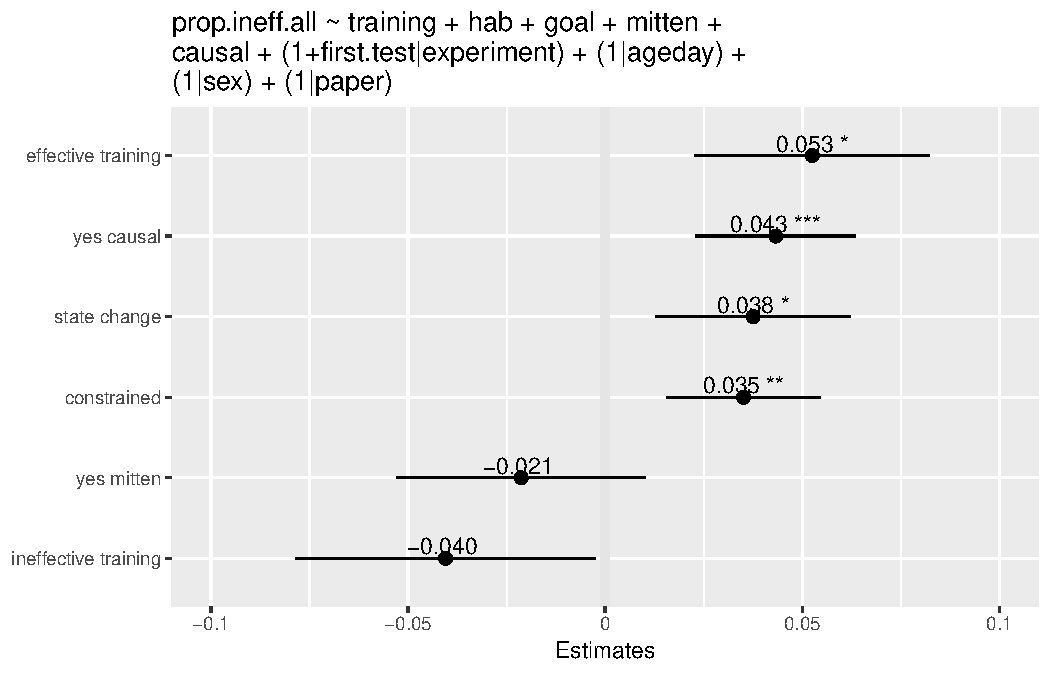
\includegraphics{lumi_analysis_files/figure-latex/meta_figure-1.pdf}
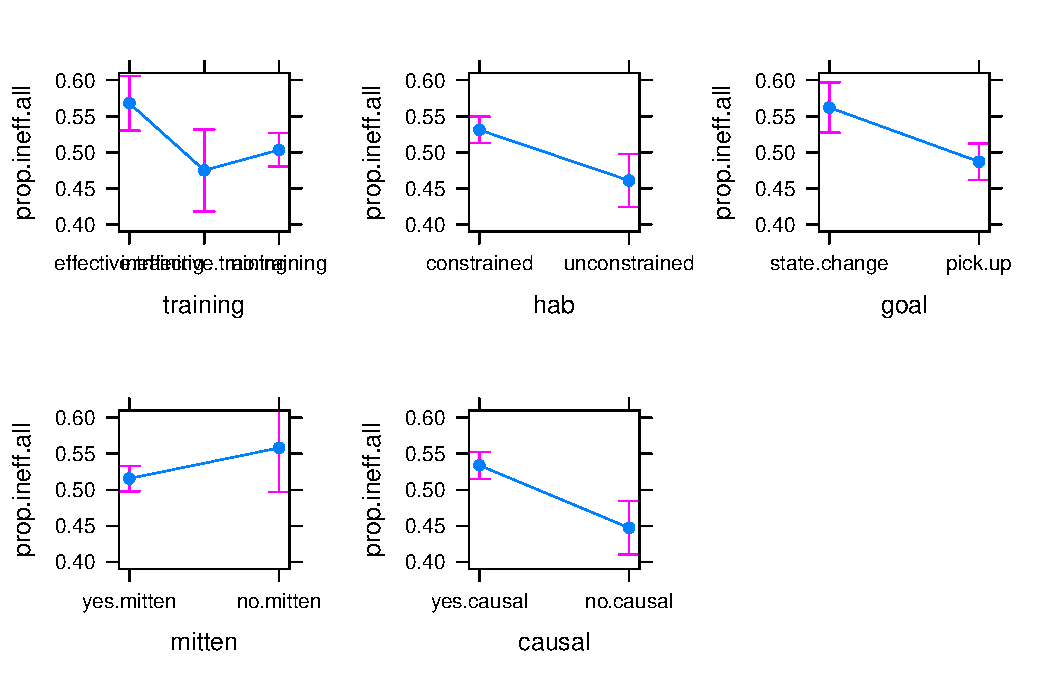
\includegraphics{lumi_analysis_files/figure-latex/meta_figure-2.pdf}

\textbf{Figure 3.} (A) Regression table and (B1-2) effect plots for
model investigating predictors of sensitivity to action efficiency
across Experiment 1-5 and all experiments from Skerry et al. (2013)
(total N=264). Dependent measure is proportion looking towards the
inefficient reach, averaged across 3 test trials during test.
Categorical predictors were coded using sum contrasts, and fixed effects
from the model should therefore be interpreted with respect to the grand
mean (with respect to 0, in (B). Error bars indicate 95\% confidence
intervals. B1 shows the effect of different manipulations relative to
the grand mean. B2 shows estimates of effects at each level of all
categorical predictors.

\begin{center}\rule{0.5\linewidth}{\linethickness}\end{center}

We found that infants' expectations were made stronger when:

\begin{itemize}
\tightlist
\item
  the action being tested was causally contingent, B=0.043,
  p=1.593\times 10\^{}\{-4\}
\item
  infants received effective motor training, relative to no training
  B=0.053, p=0.013
\item
  they were habituated to an agent whose actions were constrained,
  B=0.035, p=0.002
\item
  the person pursued a state change (vs a pickup) goal, B=0.038, p=0.025
\end{itemize}

We also found that infants' expectations were not affected when:

\begin{itemize}
\tightlist
\item
  they received ineffective motor training, relative to no training,
  B=-0.04, p=0.081
\item
  the person wore a mitten, B=-0.021, p=0.234
\end{itemize}

These results are consistent with our general interpretation infants
expect any intentional, rational agent to reach efficiently so long as
the causal mechanism of their action is clear. Either providing
pre-reaching infants with motor training or presenting them with
causally transparent actions helps them towards the insight that
reaching is a causal, intentional action.


\end{document}
